\chapter{Results}

In this chapter, the results of the previously described algorithms will be discussed. Generally, all black lines are drawn with the rake down, and the red lines are the connection paths where the BeachBot is driving with the rake in upper position.

\section{Line Drawings}

Line drawings consist of no filled areas. These types of drawings are easily created manually and therefore we have used them extensively during testing. The solutions of the manual drawings (with manual connections) are now compared to the solutions generated by the algorithm.

\subsubsection{The Lion Drawing}

The lion was one of the earliest drawings that the BeachBot was able to reproduce on the beach canvas. It is also available as part of the distributed source of the application (\texttt{assets/lion\_example.svg}).

\begin{figure}
\begin{subfigure}[b]{0.45\textwidth}
	\includegraphics[width=\textwidth]{images/results/lion/lion_handmade.pdf}
	\caption{Lion drawing created manually}
\end{subfigure}
\begin{subfigure}[b]{0.45\textwidth}
	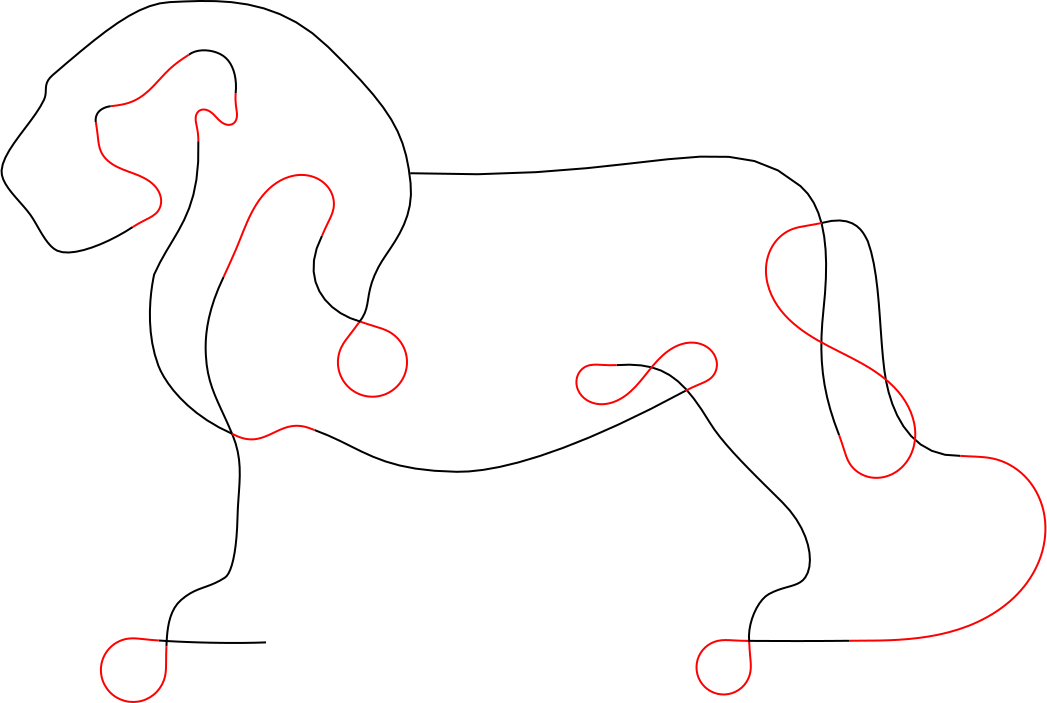
\includegraphics[width=\textwidth]{images/results/lion/lion_generated_2.pdf}
	\caption{Generated by the generator algorithm}
\end{subfigure}
\begin{subfigure}[b]{0.45\textwidth}
	\includegraphics[width=\textwidth]{images/results/lion/lion_generated_enforced_connections.pdf}
	\caption{Generated, with enforcement of one connection (blue).}
\end{subfigure}
\begin{subfigure}[b]{0.45\textwidth}
	\includegraphics[width=\textwidth]{images/results/lion/lion_generated_enforced_connections_degen.pdf}
	\caption{Generated, with two enforced connections. Since the spiro heuristic is not yet perfect, there is one unfortunate case visible}
\end{subfigure}

\caption{Comparison of manual and automatically generated lion trajectory}
\end{figure}

\subsection{The Shark Drawing}

